\que{Интеграл Бернулли. Применение интеграла Бернулли для несжимаемой жидкости в поле силы тяжести. Задача Торричелли}

\begin{theorem}
  Если для идеальной жидкости выполнены следующие условия:
  \begin{enumerate}
    \item принята модель установившихся процессов;
    \item массовые силы обладают потенциалом, т.е. $\exists \chi : \mathbf{f} = \nabla \chi$;
    \item имеет место хотя бы одно из следующих условий:
      \begin{enumerate}
        \item течение отсутсвует, т.е. $\mathbf{v} \equiv 0$;
        \item движение безвихревое, т.е. $\mathbf{\omega} = \nabla \times \mathbf{v} \equiv 0$;
        \item движение винтовое, т.е. векторы $\mathbf{\omega}$ и $\mathbf{v}$ коллинеарны:
          $\mathbf{\omega} = k \mathbf{v}$;
        \item расматривается линия тока $\mathcal{L}$, для которой $d\mathbf{x} = \mathbf{v} \, d\tau$;
        \item рассматривается вихревая линия $\mathcal{L}$, для которой $d\mathbf{x} = \mathbf{\omega} \, d\tau$,
      \end{enumerate}
  \end{enumerate}
  тогда уравнение движения допускает следующее решение (первый интеграл, называемый 
  \emph{интегралом Бернулли}): в конфигурации $\mathcal{K}$ вдоль несамопересекающейся кривой
  $\mathcal{L}$ имеет место соотношение
  \[
    \dfrac{|\mathbf{v}|^2}{2} + \mathcal{P}(p, \mathcal{L}) - \chi = i^* (\mathcal{L}),
  \]
  где $i^*$ -- некоторая константа.

  Причём:
  \begin{itemize}
    \item для первых трёх случаев $i^*$ имеет одно и тоже значение во всей рассматриваемой области
      $V$, а $\mathcal{L}$ -- произвольная кривая;
    \item для четвёртого (пятого) случая это соотношение имеет место только вдоль $\mathcal{L}$,
      которая является линией тока (вихревой линией), константа $i^*(\mathcal{L})$ сохраняет 
      своё значение только вдоль одной и той же $\mathcal{L}$, а при переходе к другой линии тока
      (вихревой линии) её значение меняется.
  \end{itemize}
\end{theorem}

\paragraph{Применение интеграла Бернулли для несжимаемой жидкости в поле сил тяжести.}
Если $\mathbf{f} = - g_\Sigma \bar{\mathbf{e}}_3$, то $\chi = - g_\Sigma s + \operatorname{const}$,
где $s = |\mathbf{x} - \mathbf{x}_\Sigma|$ -- расстояние от точки $\mathbf{x}$ до её проекции
на поверхность Земли.

Тогда интеграл Бернулли (вдоль какой-нибудь линии тока) принимает вид:
\[
  \dfrac{v^2}{2} + \dfrac{p}{\mathring{\rho}} + g_\Sigma x^3 = \dfrac{v_1^2}{2} + \dfrac{p_1}{\mathring{\rho}} + g_\Sigma x_1^3
\]

\paragraph{Задача Торричелли.} Эта задача является частным случаем предыдущего параграфа,
некоторая несжимаемая жидкость находится в сосуде с дыркой где-то снизу, этот сосуд достаточно
большой, а дырка достаточно маленькая, тогда вода на верхней поверхности жидкости почти не
движется, когда из дырки она вытикает, т.е. можно сказать что это установившийся процесс.
\begin{figure}[H]
  \centering
  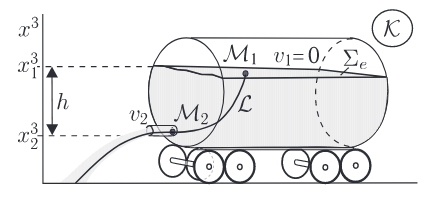
\includegraphics[width=0.9\linewidth]{img/torrichelli.png}
  \caption{Иллюстрация к задаче Торричелли.}
\end{figure}

Тогда из формулы интеграла Бернулли для несжимаемой жидкости в поле сил тяжести, где $v_1 = 0$
(на поверхности), $x^3_1 = h$, получаем
\[
  v_2 = \sqrt{ \dfrac{2p_2 - p_1}{\mathring{\rho}} + 2 g_\Sigma h }.
\]

Если $p_1 = p_2$, то получаем формулу Торричелли:
\[
  v_2 = \sqrt{2 g_\Sigma h}.
\]
